\chapter{Analogy-preserving functions}
\label{CHAP:analogy_preserving_functions}
\localtableofcontents*
\vspace*{\baselineskip}

\initial{W}e first introduced the analogical inference principle in Chapter
\ref{CHAP:formal_analogical_proportions}. This principle states that if four
elements are in analogy, then their classes (or any relevant attribute) should
also be in proportion. This is of course an unsound inference principle, in
that the conclusion does not always follow from the premises. Nonetheless, we
have seen in Chapter \ref{CHAP:functional_definition} that it can still be used
to design some classifiers that we have named conservative and extended
classifiers.  Both in \cite{BayMicDelIJCAI07} and in our experiments in Section
\ref{SEC:experiments_and_empirical_validation}, these classifiers
showed promising results, but were still only used in artificial Boolean
classification problems. Analogical classifiers still had to prove their worth
in real-world applications, and this was precisely the purpose of the previous
chapter, where we designed various techniques to apply analogical inference on
a recommendation task.

Unfortunately, the results of a direct application of the analogical inference
principle did not quite live up to our expectations. The conclusion of the last
chapter offered a partial explanation to these modest results, stating that
there were just too few decent analogies to be found in the datasets that we
used. Even if this argument is perfectly admissible, we cannot spare ourselves
the very questioning of the analogical inference principle. We say that if
four elements are in proportion then so are their classes... But why should it
even be true? Actually, this question of \textit{why} will probably be best
answered by philosophers, rather than by computer scientists. We can however
answer the question of \textit{when}: when is the analogical inference
principle sound? Said differently, what are the conditions on the function $f$
so that the inference
$$
\inferrule{\mathbf{a} : \mathbf{b} :: \mathbf{c} : \mathbf{d}}{ f(\mathbf{a}) :
f(\mathbf{b}) :: f(\mathbf{c}) : f(\mathbf{d})}
$$
is sound? The current chapter will be devoted to this question, in a Boolean
setting.

It is actually pretty easy to build up simple problems where the application of
our analogical inference principle leads to disastrous results.  Take for
example the problem of Figure \ref{FIG:classif_in_R2}. We have a set $S$ of
points (on the left) that belong to two classes that are linearly separable: an
instance is a square if it is on the left side of the space, else it is a
circle. A naive application of the analogical inference principle would lead us
to believe that for any element that is in proportion with a $3$-tuple in $S^3$
(i.e. the element is the fourth vertex of a parallelogram that we can build
with three elements in $S$), then the classes of the four vertices are in
proportion. In the right figure, we show all these elements, along with their
estimated classes. The result is absolutely terrible, because the whole space
is covered with instances belonging to both classes. In this example,
an analogical classifier would lead to very poor accuracy results.

\begin{figure}
\centering
\begin{subfigure}{.5\textwidth}
  \centering
  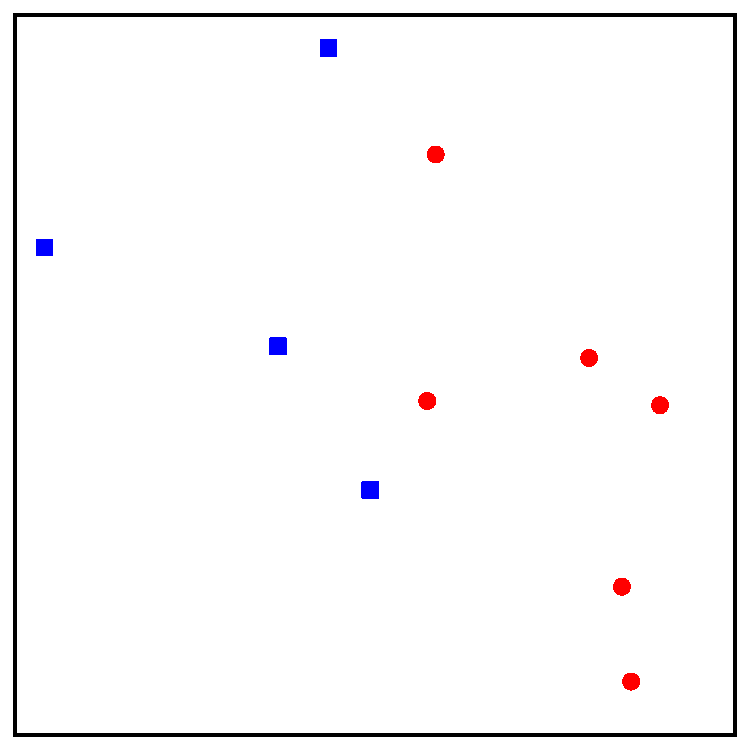
\includegraphics[width=.6\linewidth]{figures/AE_in_R2_S.pdf}
  \label{fig:sub1}
\end{subfigure}%
\begin{subfigure}{.5\textwidth}
  \centering
  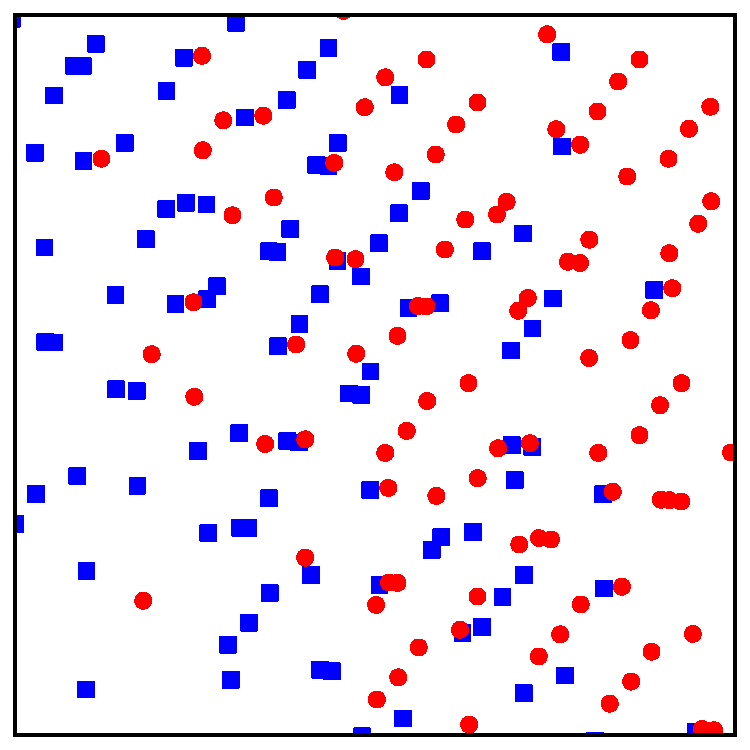
\includegraphics[width=.6\linewidth]{figures/AE_in_R2_AE.pdf}
  \label{fig:sub2}
\end{subfigure}
  \caption{A naive application of the analogical inference principle in
  $\mathbb{R}^2$.}
\label{FIG:classif_in_R2}
\end{figure}

But if it is so easy for our analogical inference principle to fail, then why
does it work well in some other cases? Back to Figure \ref{FIG:nan_vs_nn} on
page \pageref{FIG:nan_vs_nn}, the accuracies of the NAN algorithm were
definitely not as bad as that of the problem we have just seen, and some of
them were actually really good. A first obvious difference between the two
experiments is that the one we just described deals with the arithmetic
proportion with real-valued instances, while the other one deals with Boolean
attributes. Does it mean that the analogical inference principle is bound to
fail with the arithmetic proportion? We will probably not be able to completely
answer this question, even though we will provide some insights.  We will
instead focus on the Boolean setting which has seemed to be the most promising
for analogical inference so far, and from there we will derive some links with
the real-valued case.

In this chapter, we will provide a complete characterization of functions that
are fully compatible with the analogical inference principle in a Boolean
setting. Let us restate the inference principle in this context to explain what
we mean: for any four elements $\mathbf{a}, \mathbf{b}, \mathbf{c}, \mathbf{d}$
in $\mathbb{B}^m$, the analogical inference principle states that if
$\mathbf{a}: \mathbf{b}:: \mathbf{c}: \mathbf{d}$ holds, then $f(\mathbf{a}):
f(\mathbf{b}):: f(\mathbf{c}): f(\mathbf{d})$ also holds, where $f$ is a Boolean function
from $\mathbb{B}^m$ to $\mathbb{B}$. We have said it before:  this principle is
unsound. The goal of this chapter is to identify all of the functions $f$ that
lead to a valid conclusion, i.e. the functions such that $\mathbf{a}:
\mathbf{b}:: \mathbf{c}: \mathbf{d} \implies f(\mathbf{a}):f(\mathbf{b})::
f(\mathbf{c}): f(\mathbf{d})$ (with some minimal and natural requirements). We
will say that these functions are \textbf{analogy preserving} (AP).

We will tackle this problem by adopting the general point of view of  the
training set extension. In Section \ref{SEC:extending_a_training_set}, we will first
define the problem of training set extension, describe some previous works and
explain how this problem can motivate the research of analogy preserving
functions. In Section \ref{SEC:a_complete_characterization_of_AP_functions}, we
will
give a complete and accurate depiction of analogy preserving functions by
showing that the class of analogy preserving functions is the class of
(Boolean) affine functions. This strong theoretical result will be complemented in
Section \ref{SEC:beyond_boolean_AP_functions}, where we will study some functions that
derive from AP in various ways. We also address the identification of AP
functions in a nominally valued setting and in a real setting, where we will
once again witness the close links between the Boolean proportion and the
arithmetic proportion.

\section{Extending a training set}
\label{SEC:extending_a_training_set}

We have proved in Chapter \ref{CHAP:functional_definition} that the analogical
classification process can be formalized via two new conceptual steps:
\begin{enumerate}
  \item First, the analogical extension $\esf$ of the training set is computed. This
    extension is the set of all elements in the instance space that are in
    analogy with one $3$-tuple in the training set, provided that the
    associated class equation is solvable. Each element of the extension is
    associated with an estimated label: the analogical label denoted $\albl{x}$.
  \item Then, a $k$-NN algorithm is run, considering that the training set is
    now the analogical extension. This $k$-NN classifier allows to
    classify all the elements of the universe that are not in the analogical
    extension.
\end{enumerate}

But then a natural question arises: why should we stick to a $k$-NN classifier?
The reason why the $k$-NN algorithm is used is because in their algorithmic
description, extended learners rely on an analogical dissimilarity, which is
strongly related to a distance on the instance space. But now that we have an
equivalent definition of extended classifiers that does not rely explicitly on
an analogical dissimilarity, nothing actually prevents us from using any other
classifier such as a decision tree, a support vector machine, or any of the
dozens of learners available out there. This would lead us to a different
paradigm for analogical learning: you first extend the training set by building
the analogical extension, and then you are free to do how you please and use
this extension as a bigger training set with any classifier.

In the next subsection, we will formally describe the problem of training set
extension, and present some previous works on this subject. Then in subsection
\ref{SEC:analogy_preserving_presentation}, we will introduce the class of
analogy preserving functions, which lead to a perfectly sound training set
extension in all cases.

\subsection{Previous works on training set extension}

Machine learning algorithms usually require training on sufficiently large
datasets. The problem of learning from few examples is not new and is
referred-to as one-shot learning, where we rely on a transfer of knowledge from
known classes to unknown classes: see  for example \cite{LiFerPerPAMI06} in a
pattern recognition context.  But other options are available when the number
of training instances is small, and training set extension naturally comes in
as a handy tool. Indeed, the extension of the training set is a simple idea to
improve the generalization power of the learner.  The more examples you have, the
better you learn! The point is here to add to the training set $S$ some new
examples, and to try do that in a way that preserves the \textit{quality} of
$S$.

Formally, we start with a set $S= \{\mathbf{x}^{(i)} \in X^m| i \in
[1,n]\}$ of examples ($n$ is supposed to be small), where $\mathbf{x}^{(i)}$ is
an element of a Cartesian product $X^m = X_1 \times \ldots \times X_m$.
For each element  $\mathbf{x}^{(i)} \in S$, we associate a target
$f(\mathbf{x}^{(i)})=y^{(i)} \in Y$.  In the case of regression $y^{(i)} \in
\mathbb{R}$, and in the case of classification $y^{(i)}$ belongs to a finite
set.

Actually, only a few methods have been proposed for extending a training set with
new examples, and most of them are specific to a particular application. For
example in \cite{CanPerArlLlo06}, some techniques are proposed but they are
only relevant for character recognition tasks. In the general case, we may
consider that we can build a new example starting from 1, 2 or 3 known
examples.
\begin{enumerate}
\item With one example, a natural way to proceed is to use the classical
  neighborhood approach: given one  example $(\mathbf{a},f(\mathbf{a}))$, we
    can generate a new example $(\mathbf{b},f(\mathbf{b}))$ where  $\mathbf{b}$
    is not too far from $\mathbf{a}$ and $f(\mathbf{b})$ is not too far from
    $f(\mathbf{a})$. In the classification case, $f(\mathbf{b})$ may be chosen
    as $f(\mathbf{a})$. This is the setting in which \cite{CanPerArlLlo06}
    operates, where new characters are generated by slanting, shrinking, and
    dilating of training instances.
\item With two examples, the previous neighborhood option is still available
  and leads to interpolate the new example from the two given ones.  A somehow
    different option is the Feature Knockout procedure \cite{WolMar04}, which
    amounts to build a third example obtained by modifying a randomly chosen
    feature of the first example with that of the second one.  This way to
    proceed enjoys nice properties and appears to be equivalent to the popular
    Tikhonov regularization  technique in the case of linear regression (also
    known  as Ridge regression).  A
    related idea is used in a recent proposal \cite{BouPraRicECAI16} which
    introduces a measure of oddness with regard to a class that is computed on the
    basis of pairs made of two nearest neighbors in the same class; this is
    equivalent to replacing the two neighbors by a fictitious representative of
    the class.

\item With three examples $(\mathbf{a},f(\mathbf{a})),
  (\mathbf{b},f(\mathbf{b})), (\mathbf{c},f(\mathbf{c}))$, the previous options
    remain available and lead to build a fourth example which is somehow
    in-between the three other ones: we still have some kind of interpolation.
    A quite different idea is to extrapolate the fourth item on the basis of
    analogical proportions.  In this perspective, this fourth element is not
    necessarily in the neighborhood of the three others. In fact, this idea has
    been addressed in \cite{BayMouMicAnqECML07}, where the authors generated
    new examples that had the least analogical dissimilarity with some
    $3$-tuples in $S^3$. The analogical dissimilarity was an AD between
    sequences, and they used it to generate new examples of handwritten
    characters modeled using the Freeman coding, which is a sequence of symbols
    indicating the successive directions of the pen that are needed to write
    the character. They used their extended training set to train an SVM and a
    Radial Basis Function Network for a classification task, and results showed
    that the classifiers had better results when they were trained with the
    analogically-extended training set than when they were trained with an
    extended training set using other generation techniques (such as those of
    \cite{CanPerArlLlo06}).  Note though that just like the algorithmic
    description of the extended classifier using analogical dissimilarity, we
    here only have an algorithmic description of this training set extension
    procedure. The authors in \cite{BayMouMicAnqECML07} never explicitly refer
    to the analogical extension set $\esf$, and this is normal because the
    unifying framework between the works in \cite{BayMicDelIJCAI07} and the
    works in \cite{StrYvoCNLL05} were only made later in
    \cite{HugPraRicSerECAI16}, as described in Chapter
    \ref{CHAP:functional_definition}.
\end{enumerate}


As far as we know, the problem of generation of new examples has never been
addressed from a theoretical point of view (except for the Knockout procedure,
which is only relevant in some particular settings), and this is actually quite
understandable. Before they can be used in an extended training set, the new
generated examples have to be assigned an estimated label... But how do we
estimate these labels? Well there is a name for such problems: it is called
classification, and classification was the actual reason why we wanted to
extend the training set in the first place, so we have a vicious circle here.
In some sense, extending a training set with potentially noisy data
amounts to nothing but performing classification on a specific set of
instances.

However, training set extension can still be extremely useful if we are
perfectly sure that the new added examples are sound, i.e. that their estimated
labels are the correct ones. In the next subsection, we will formally define
this problem in the context of analogical learning. Section
\ref{SEC:a_complete_characterization_of_AP_functions} will then be devoted to
the identification of the cases where such a perfect extension is feasible.

\subsection {Analogy preserving functions: a safe way to extend a training set}
\label{SEC:analogy_preserving_presentation}

In the rest of this chapter, we will address the problem of extending a
training set using analogical proportions in a Boolean setting. Instead of
using an analogical dissimilarity like in  \cite{BayMouMicAnqECML07}, we will
use our equivalent
functional framework described in Chapter \ref{CHAP:functional_definition},
i.e. we will consider that the extension of the training set $S$ is the
analogical extension $\esf$, where $f$ is the function underlying the ground
truth labels. Algorithmically, the generation of $\esf$ and the computation of
the analogical labels goes as follows:
\begin{enumerate}
  \item Add every $\mathbf{x} \in S$ to $\esf$. Then, for every
    $\mathbf{a},\mathbf{b},\mathbf{c} \in S$ such that $f(\mathbf{a}) :
    f(\mathbf{b}) :: f(\mathbf{c}) : y$ is solvable and such that there is
    $\mathbf{x} \in \mathbb{B}^m \setminus S$ with $\mathbf{a} : \mathbf{b} ::
    \mathbf{c} : \mathbf{x}$, add $\mathbf{x}$ to $\esf$ and save
    the solution $\sol(f(\mathbf{a}), f(\mathbf{b}), f(\mathbf{c}))$ as a candidate
    for $\albl{\mathbf{x}}$.
\item Then for every $\mathbf{x} \in \esfs \eqdef \esf \setminus S$, run a
  \textbf{majority-vote procedure}: set $\albl{\mathbf{x}}$ as the most
    common candidate among all solutions $\sol(f(\mathbf{a}), f(\mathbf{b}),
    f(\mathbf{c}))$ where $(\mathbf{a}, \mathbf{b}, \mathbf{c})$ is in the
    analogical root of $\mathbf{x}$. In case of a tie between two labels, then
    one of the values is chosen at random.  For elements in $S$,
    $\albl{\mathbf{x}}$ is simply set to $f(\mathbf{x})$.
\end{enumerate}

\noindent
The extension $\esf$ is then considered to be an extended training set, where
the labels are the analogical labels, \textbf{which are not necessarily
correct}. Indeed
for some elements $\mathbf{x} \in \esfs$, it may happen that
$\albl{\mathbf{x}} \neq f(\mathbf{x})$, simply because the analogical inference
principle may not be \textit{suitable} for the function $f$. In this chapter,
we  are precisely interested in the identification of all Boolean functions $f$
that lead to perfectly sound extensions, i.e. extensions where the analogical
labels $\albl{\mathbf{x}}$ are always equal to the ground truth values
$f(\mathbf{x})$. These functions will be called \textbf{Analogy preserving}
functions:

\begin{definition}[Analogy preserving functions]
  We say that $\esf$ is {\bf sound} if
  $\albl{\mathbf{x}}=f(\mathbf{x})$ for every $\mathbf{x} \in
  \esfs$. In other words, $\esf$ is sound if $\omegasf
  \eqdef P\left(\albl{\mathbf{x}} = f(\mathbf{x}) \given[\big] \mathbf{x} \in
  \esfs\right) = 1$.

  \noindent
  Also, if $\esf$ is sound for all $S \subseteq
  \mathbb{B}^m$, we say that $f$ is {\bf Analogy Preserving} (AP).
\end{definition}

\noindent
Proposition \ref{PROPOS:equivalent_def_AP} gives an equivalent definition of AP
functions, that will be more useful to convey our proofs:

\begin{proposition}
  \label{PROPOS:equivalent_def_AP}
  A function $f \colon \mathbb{B}^m \to \mathbb{B}$ is AP iff for every
  $\mathbf{a}, \mathbf{b}, \mathbf{c}, \mathbf{d} \in \mathbb{B}^m$, $f$ suits
  the following requirement:
  $$
  \begin{cases}
    \mathbf{a} :  \mathbf{b} ::  \mathbf{c} :  \mathbf{d} \emph{ and }\\
    \emph{solvable}(f(\mathbf{a}), f(\mathbf{b}),  f(\mathbf{c}))
  \end{cases}
  \implies \emph{sol}\left(f(\mathbf{a}),  f(\mathbf{b}),  f(\mathbf{c})\right) =
  f(\mathbf{d}). $$
\end{proposition}
\begin{proof}
  If $f$ fulfills  this requirement, then it is clear from the algorithmic
  description given above that for any $S \subseteq \mathbb{B}^m$ and
  $\mathbf{x} \in \esfs$, all the candidates for $\albl{\mathbf{x}}$ are equal
  to $f(\mathbf{x})$, so $\albl{\mathbf{x}}$ will be invariably set to
  $f(\mathbf{x})$ by the majority-vote procedure, which makes $f$ AP.

If $f$ does not suit this requirement, then there exist $\mathbf{a},
  \mathbf{b}, \mathbf{c}$, and $\mathbf{d} \in \mathbb{B}^m$ such that
  $\mathbf{a} : \mathbf{b} :: \mathbf{c} : \mathbf{d}$ but the solution
  $\sol(f(\mathbf{a}), f(\mathbf{b}), f(\mathbf{c}))$ is not equal to
  $f(\mathbf{d})$. Taking $S_0 = \{\mathbf{a}, \mathbf{b}, \mathbf{c}\}$ we
  obtain $\mathbf{E}^{f*}_{S_0} = \{\mathbf{d}\}$, and since $\albl{\mathbf{d}}
  = \sol(f(\mathbf{a}), f(\mathbf{b}), f(\mathbf{c})) \neq f(\mathbf{d})$, then
  $\mathbf{E}_{S_0}^f$ is not sound so $f$ is not AP.
\end{proof}

\noindent
It should be clear from Proposition \ref{PROPOS:equivalent_def_AP} that looking
for the functions that lead to a perfect extension (i.e. the AP functions) is
equivalent to looking for the functions that are compatible with the analogical
inference principle, which was the first purpose of this chapter. Indeed,
saying that $\sol\left(f(\mathbf{a}),  f(\mathbf{b}),
f(\mathbf{c})\right) =f(\mathbf{d})$ is equivalent to saying that
$f(\mathbf{a}) : f(\mathbf{b}) ::  f(\mathbf{c}) :  f(\mathbf{d})$.

Let us note that many natural functions are not AP. Consider for example the
binary function $f(x_1,x_2)= x_1 \wedge x_2$, along with $\mathbf{a},
\mathbf{b}, \mathbf{c}, \mathbf{d} \in \mathbb{B}^2$ in Table
\ref{exampleNotAP}.  We have $\mathbf{a} : \mathbf{b} :: \mathbf{c} :
\mathbf{d}$ and $f(\mathbf{a}) : f(\mathbf{b}) :: f(\mathbf{c}) : y$ is
solvable, yet the solution is $\sol(f(\mathbf{a}), f(\mathbf{b}),
f(\mathbf{c}))=0$, which  is different from $f(\mathbf{d})=1$ so $f$ is not AP.
This actually comes from the fact that analogical proportions are not stable by
conjunction combination. It is also the case for the disjunction
\cite{PraRic14}.

\begin{table}[ht]
  \center
$\begin{array}{cccc}
  \toprule
  ~ & x_1 & x_2 & f(\cdot) \\
  \midrule
  \mathbf{a} & 0 & 0 & 0\\
  \mathbf{b} & 0 & 1 & 0\\
  \mathbf{c} & 1 & 0 & 0\\
  \mathbf{d} & 1 & 1 & 1\\
  \bottomrule
\end{array}
$\bigskip
\caption{$f(x_1,x_2)= x_1 \wedge x_2$ is not AP.}
\label{exampleNotAP}
\end{table}

The following section will be devoted to a complete characterization of AP
functions in a Boolean setting.

\section{A complete characterization of analogy preserving functions}
\label{SEC:a_complete_characterization_of_AP_functions}

We will show in this section that the class of AP functions is the class of
affine functions, which will be defined later. To complete our proofs, we will
first need to recall some background knowledge on Boolean algebra and Boolean
functions, which is the purpose of the next subsection.

\subsection{Preliminary background on Boolean functions}

Our first step will be to use a unifying notation for all of the Boolean
functions, and to adopt an algebraic point of view.  In the following, the AND
operator `$\wedge$' will be denoted `$\cdot$', and `$+$' will now denote the
modulo-2 addition, equivalent to the XOR operator.  We shall make use of the
polynomial representation of Boolean functions, that we now describe. A
\textbf{ monomial} is a term of the form:
$$\mathbf{x}_I=\underset{i\in I}{\prod}x_i,$$ for some possibly empty finite
set of positive integers $I$, where $|I|$ is called the \textbf{degree} of
$\mathbf{x}_I$. Simply put, a monomial is a conjunction of variables. We take
the convention that $1$ is the empty monomial $\mathbf{x}_\emptyset $. A
\textbf{ polynomial} is a sum of monomials and its degree is the largest degree
of its monomials.  It is well-known \cite{StoneAlgebra36,ZhegalkinAlgebra27}
that \textbf{any function $f:\mathbb{B}^m\rightarrow \mathbb{B}$ is uniquely
represented by a polynomial}, also called the \textbf{Algebraic Normal Form}
(ANF) of $f$:
$$f(x_1,\ldots,x_m)=\sum_{I\subseteq \{1,\ldots,m\}}a_I\cdot \mathbf{x}_I,$$
where each $a_I$ belongs to $\mathbb{B}$. The degree of a function $f:\mathbb{B}^m\rightarrow
\mathbb{B}$, denoted $d(f)$, is defined as the degree of the unique polynomial
representing $f$. In the following, we will often refer to $f$ as both a
function object and as the associated ANF.

\begin{testexample}
To illustrate this concept, here are
the ANF of some common Boolean functions in $\mathbb{B}^2$ or $\mathbb{B}$:

\begin{itemize}
  \item $\text{AND}(x_1, x_2) = x_1 \cdot x_2$;
  \item $\text{OR}(x_1, x_2) = x_1 + x_2 + x_1 \cdot x_2$;
  \item $\text{XOR}(x_1, x_2) = x_1 + x_2$;
  \item $\text{NEG}(x_1) = x_1 + 1$;
  \item The constant function $f(x_1, x_2) = 0$ is represented by
    $a_\emptyset\cdot \mathbf{x}_\emptyset$ with $a_\emptyset =0$. The constant
    function $f(x_1, x_2) = 1$ is also represented by $a_\emptyset\cdot
    \mathbf{x}_\emptyset$, but this time $a_\emptyset =1$.
\end{itemize}
\end{testexample}

Another key concept of our proof is the notion of essential and inessential
variables.  For $k\in [1,m]$, $\boldsymbol{\alpha}\in \mathbb{B}^m$, and $c \in
\mathbb{B}$, let ${\boldsymbol{\alpha}}_{k}^c$ be the tuple in $\mathbb{B}^{m}$
whose $i$-th component is set to $c$ if $i=k$, and to $\alpha_i$ otherwise.  A
variable $x_i$ is said to be \textbf{inessential} in $f\colon \mathbb{B}^m\to
\mathbb{B}$ if for all $\boldsymbol{\alpha} \in \mathbb{B}^m$ and $c \in
\mathbb{B}$, $f(\boldsymbol{\alpha}^c_i) = f(\boldsymbol{\alpha}^{\neg c}_i)$.
Otherwise, $x_i$ is said to be \textbf{essential} in $f$, or that $f$ depends
on $x_i$. In simple terms, an essential variable is a variable that has the
\textit{ability} to change the value of $f$. In fact, it can be shown that if
$x_i$ is an inessential variable for a function $f$, then $x_i$ does not appear
in the ANF of $f$.  For example in $f(x_1, x_2, x_3) = x_1 \cdot x_3$, $x_1$
and $x_3$ are essential variables while $x_2$ is inessential.  We denote by
$\ess(f)$ the number of essential variables of $f$ (or \textbf{essential
arity}).

Two functions $f\colon \mathbb{B}^m\to \mathbb{B}$ and $g\colon \mathbb{B}^n\to
\mathbb{B}$ are said to be {\bf equivalent} if there exist two mappings
$\sigma\colon
[1,n]\to [1,m]$ and $\sigma'\colon [1,m]\to [1,n]$ such that:
\begin{align*}
  f(x_1,\ldots , x_m)&=g(x_{\sigma(1)},\ldots,x_{\sigma(n)}) \text{ and} \\
   g(x_1,\ldots , x_n)&=f(x_{\sigma'(1)},\ldots,x_{\sigma'(m)}).
\end{align*}
In other words, $f$ and $g$ are equivalent if one can be obtained from the
other by permutation of variables, addition of inessential variables, or
identification of inessential variables. Another point of view is to consider
that two functions are equivalent if their ANF is the same, up to the
renaming of variables. For example, $f(x_1, x_2, x_3) = x_1
\cdot x_3$ and $g(x_1, x_2)  = x_1 \cdot x_2$ are equivalent functions.  Two
equivalent functions necessarily have the same number of essential
variables. For further background on the theory of essential variables of
functions, see \cite{CouceiroTCS08, CouceiroDM09, SalomaaAASF63, WillardDM96}.
In our demonstrations, we will use the following property:

\begin{property}\label{equivalent_functions}
Let $f\colon \mathbb{B}^m\to \mathbb{B}$ and $g\colon \mathbb{B}^n\to
  \mathbb{B}$ be equivalent functions. Then $f$ is AP if and only if $g$ is AP.
\end{property}

This can be verified by noting that as the analogy in $\mathbb{B}^m$ is defined
in a component-wise fashion, the permutation of variables has no effect on the equation and
its solution. Also, manipulation of inessential variables does not change the
value of the function $f$, and thus the AP property still holds.

We now define the concept of \textbf{section} of a function, also known as a
\textit{restriction}, or equivalently as the result of \textit{partial
application} in computer science. Let $f$ be a function $\mathbb{B}^m\to
\mathbb{B}$, and $(I, J)$ be a partition of $[1, m]$. With $\mathbf{x} \in
\mathbb{B}^m$ and $\boldsymbol{\alpha} \in \mathbb{B}^{|I|}$, the $I$-section
(or simply section) $f^{\boldsymbol{\alpha}}_I \colon \mathbb{B}^{|J|} \to
\mathbb{B}$ is the function that is obtained after setting all variables in $I$
to the components of $\boldsymbol{\alpha}$.  More formally, let us define
$(\mathbf{x}^{\boldsymbol{\alpha}}_I) \in \mathbb{B}^m$ as follows:
$$
\begin{cases}
(\mathbf{x}^{\boldsymbol{\alpha}}_I)_i \eqdef x_i \mbox{ if } i \notin I\\
(\mathbf{x}^{\boldsymbol{\alpha}}_I)_i \eqdef \alpha_j \mbox{ where } j \mbox{
  is the index of } i \mbox{ in } I.
\end{cases}
$$
Concretely, $\mathbf{x}^{\boldsymbol{\alpha}}_I$ is nothing but the vector $\mathbf{x}$
where the components at the  indices in $I$ have been replaced by the
successive components of $\boldsymbol{\alpha}$. For instance, with $m=5,
\mathbf{x}=(0,1,1,0,0), I=\{1,3,4\}$ and $\boldsymbol{\alpha}=(1,0,0)$, we
have $(\mathbf{x}^{\boldsymbol{\alpha}}_I)=(1,1,0,0,0)$.  The $I$-section
$f^{\boldsymbol{\alpha}}_I$ is the function from $\mathbb{B}^{\mid J \mid} \to
\mathbb{B}$ defined as:
$$\forall \mathbf{y} \in \mathbb{B}^{|J|},~~
f^{\boldsymbol{\alpha}}_I(\mathbf{y}) \eqdef
f((\mathbf{x}^{\boldsymbol{\alpha}}_I)^\mathbf{y}_J).$$
The arity of $f^{\boldsymbol{\alpha}}_I$ is $|J|$ and is always less
than the arity of $f$, and 
$\ess(f^{\boldsymbol{\alpha}}_I) \leq \ess(f)$.  As an example, let us consider
the function $f\colon \mathbb{B}^3 \to \mathbb{B}$ such as:
$$f(x_1,x_2, x_3) = x_1 \cdot x_2 \cdot x_3 + x_1 \cdot x_2 + x_3.$$
The section $f^{(1, 0)}_{\{1, 3\}}$ is a function from $\mathbb{B}$ to
$\mathbb{B}$ and is defined by $f^{(1, 0)}_{\{1, 3\}}(x_2) = x_2$.
A main result about sections that will be used in other proofs is stated in
Property \ref{section_preserve_wap}:

\begin{property}\label{section_preserve_wap}
If $f\colon \mathbb{B}^m\to \mathbb{B}$ is AP, then every section of $f$ is
  also AP.
\end{property}
\begin{proof}
  This statement is actually pretty obvious but sadly, its proof is quite ugly.
  Let $f$ be an AP function from $\mathbb{B}^m$ to $\mathbb{B}$, $(I,J)$ a
  partition of $[1, m]$, and $\boldsymbol{\alpha} \in \mathbb{B}^{|I|}$. We
  will consider the section  $f^{\boldsymbol{\alpha}}_I$.  Let us now assume
  that we have $\mathbf{a},\mathbf{b},\mathbf{c}, \mathbf{d} \in
  \mathbb{B}^{|J|}$ with the two following properties:
  $$
  \begin{cases}
    \mathbf{a}:\mathbf{b}::\mathbf{c}:\mathbf{d}\\
    \solvable(f^{\boldsymbol{\alpha}}_I(\mathbf{a}),
    f^{\boldsymbol{\alpha}}_I(\mathbf{b}),
    f^{\boldsymbol{\alpha}}_I(\mathbf{c})).
  \end{cases}
  $$
  We want to prove that this implies that
  $\sol(f^{\boldsymbol{\alpha}}_I(\mathbf{a}),
  f^{\boldsymbol{\alpha}}_I(\mathbf{b}), 
  f^{\boldsymbol{\alpha}}_I(\mathbf{c}))
  =
  f^{\boldsymbol{\alpha}}_I(\mathbf{d})$.
  First, let us note that the following property holds:
$$\forall \mathbf{a},\mathbf{b},\mathbf{c}, \mathbf{d} \in \mathbb{B}^{|J|},~J
  \subsetneq [1,m], ~ \mathbf{x} \in \mathbb{B}^m,~~ \mathbf{a}: \mathbf{b} ::
  \mathbf{c} : \mathbf{d} \implies \mathbf{x}^{\mathbf{a}}_J :
  \mathbf{x}^{\mathbf{b}}_J:: \mathbf{x}^{\mathbf{c}}_J :
  \mathbf{x}^{\mathbf{d}}_J,$$
  simply due to the fact that $\mathbf{x}:\mathbf{x}::\mathbf{x}:\mathbf{x}$
  always holds.

Regarding the first condition $\mathbf{a}:\mathbf{b}::\mathbf{c}:\mathbf{d}$,
since $\forall \mathbf{x} \in \mathbb{B}^m,$ we have that $
  \mathbf{x}^{\boldsymbol{\alpha}}_I : \mathbf{x}^{\boldsymbol{\alpha}}_I ::
  \mathbf{x}^{\boldsymbol{\alpha}}_I : \mathbf{x}^{\boldsymbol{\alpha}}_I$,
  and we
  deduce: $(\mathbf{x}^{\boldsymbol{\alpha}}_I)^{\mathbf{a}}_J :
  (\mathbf{x}^{\boldsymbol{\alpha}}_I)^{\mathbf{b}}_J ::
  (\mathbf{x}^{\boldsymbol{\alpha}}_I)^{\mathbf{c}}_J :
  (\mathbf{x}^{\boldsymbol{\alpha}}_I)^{\mathbf{d}}_J$.
By definition $f^{\boldsymbol{\boldsymbol{\alpha}}}_I(\mathbf{y}) =
  f((\mathbf{x}^{\boldsymbol{\alpha}}_I)^{\mathbf{y}}_J)$, and the second
  condition is just:
  $$\solvable(f((\mathbf{x}^{\boldsymbol{\alpha}}_I)^\mathbf{a}_J),
  f((\mathbf{x}^{\boldsymbol{\alpha}}_I)^\mathbf{b}_J),
  f((\mathbf{x}^{\boldsymbol{\alpha}}_I)^\mathbf{c}_J)).$$
  Since $f$ is AP, we have that
  $\sol(f((\mathbf{x}^{\boldsymbol{\alpha}}_I)^\mathbf{a}_J),
  f((\mathbf{x}^{\boldsymbol{\alpha}}_I)^\mathbf{b}_J),
  f((\mathbf{x}^{\boldsymbol{\alpha}}_I)^\mathbf{c}_J))=
  f((\mathbf{x}^{\boldsymbol{\alpha}}_I)^\mathbf{d}_J) \eqdef
  f^{\boldsymbol{\alpha}}_I(\mathbf{d})$,
  which is precisely the condition for
  $f^{\boldsymbol{\boldsymbol{\alpha}}}_I$ to be AP.
\end{proof}


This section was quite dense so let us recap what we have seen. We
described functions by their ANF, which is a polynomial representation. This ANF
allowed us to define the degree of a function, which has a similar meaning to
the notion of degree for real valued polynomials. We also defined the notion of
equivalent functions, and showed that two equivalent functions are either both
AP, or none of them are. Finally, we defined the section of a function which is
a function of lower arity, and saw that sectioning an AP function leads to
another AP function.

We are now in a position to examine some examples of AP functions. We will first
show that any affine function is AP, and we will then prove that these
functions are actually the only AP functions.

\subsection{The class of Analogy Preserving functions}
\label{SEC:the_class_of_AP_functions}

Let us first define the class of affine functions:
\begin{definition}[Affine functions]
  The class $L$ of \textbf{affine} functions is the set of functions $f$ of the
  form:
  $$f(x_1,\ldots , x_m)=\alpha_1\cdot x_1+\ldots +\alpha_m\cdot
  x_m+\alpha_0,$$
  where $\alpha_0,\ldots, \alpha_m$ are elements of $\mathbb{B}$. We also
  write:
  $$f(\mathbf{x}) = \boldsymbol{\alpha} \cdot \mathbf{x} + \alpha_0,$$
  where $\boldsymbol{\alpha} \in \mathbb{B}^m$ and $\cdot$ is here a scalar
  product.  If $\alpha_0= 0$, we say that $f$ is \textbf{linear}.
\end{definition}

We used the polynomial representation of the function $f$, and we can see that
$L$ is precisely the set of functions whose degree is less than or equal to
$1$. Informally, a linear function is a function that computes the exclusive OR
between any subset of variables. The class $L$ of affine functions is then the set of all linear
functions along with their negations (because $f + 1$ = $\neg f$). A particular
case of affine functions are the \textbf{projections} or \textbf{dictator}
functions, defined by $f(\mathbf{x}) = x_i + \alpha_0$. These functions will be
of interest in the next subsection.

Now, we will prove that every affine function is AP:
\begin{proposition}
  \label{PROPOS:affine_functions_are_ap}
  Any affine function $f$ is AP.
\end{proposition}

\begin{proof}
  Let $f \colon \mathbb{B}^m \to \mathbb{B} \in L$. Using the obvious fact that
  $f$ is AP  iff $f + 1 = \neg f$ is AP, we may assume without loss of
  generality that $\alpha = 0$. Also, considering that $f$ essentially depends
  on $n \leq m$ variables ($n$ is then the number of $\alpha_i$ equal to $1$),
  $f$ is equivalent to the function $g \colon \mathbb{B}^n \to \mathbb{B}$
  defined by $g(x_1, \cdots, x_n) = x_1 +  \cdots + x_n$. Using Property
  \ref{equivalent_functions}, we just need to prove that $g$ is AP to show that
  $f$ is also AP.

  This function $g$ has the remarkable property\footnote{This is the reason why
  affine functions lead to classification problems that are, in fact, highly
  \textbf{non} linearly separable.} that changing the value of any $x_i$
  changes the value of $g$: $\forall _i, \quad g(x_1, \cdots, x_i, \cdots, x_n)
  = \neg g(x_1, \cdots, \neg x_i, \cdots, x_n)$, as illustrated on Figure
  \ref{FIG:affine_functions_neighbors}. From this property, it is easy to see
  that:
  $$\forall \mathbf{x}, \mathbf{x}' \in \mathbb{B}^n, g(\mathbf{x}) =
  g(\mathbf{x}') \iff H(\mathbf{x}, \mathbf{x}') \text{ is even},$$
  where $H$ is the Hamming distance function.

  Let $\mathbf{a}, \mathbf{b}, \mathbf{c}, \mathbf{d} \in \mathbb{B}^n$  such
  that the two hypotheses in the definition of AP are satisfied, i.e.
  $$
  \mathbf{a} : \mathbf{b} :: \mathbf{c} : \mathbf{d}\quad \text{and}\quad
  g(\mathbf{a}) : g(\mathbf{b}) :: g(\mathbf{c}) : y\quad  \text{is  solvable}.
  $$

  This equation is solvable in two possible cases: either $g(\mathbf{a}) =
  g(\mathbf{b})$, or $g(\mathbf{a}) = g(\mathbf{c})$. This can be verified in
  Table \ref{TAB:six_valid_patterns} on page \pageref{TAB:six_valid_patterns},
  or by referring to Proposition \ref{PROPOS:equation_solving}.
  Also, we know from Property \ref{PROPER:hamming_distance_boolean_proportion}
  that as $\mathbf{a} : \mathbf{b} :: \mathbf{c} : \mathbf{d}$, we have
  $H(\mathbf{a}, \mathbf{b}) = H(\mathbf{c}, \mathbf{d})$ and $H(\mathbf{a},
  \mathbf{c}) = H(\mathbf{b}, \mathbf{d})$.
  Therefore, we either are in one of the two following cases:
  \begin{enumerate}
    \item $g(\mathbf{a}) = g(\mathbf{b})$, and in this case the solution is
      $\sol(g(\mathbf{a}), g(\mathbf{b}), g(\mathbf{c})) = g(\mathbf{c})$. As
      $g(\mathbf{a}) = g(\mathbf{b})$, then $H(\mathbf{a}, \mathbf{b})$ is
      even, and so is $H(\mathbf{c}, \mathbf{d})$. Then, $g(\mathbf{c}) =
      g(\mathbf{d})$, and thus $\sol(g(\mathbf{a}), g(\mathbf{b}),
      g(\mathbf{c})) = g(\mathbf{d})$.
    \item $g(\mathbf{a}) = g(\mathbf{c})$, and in this case the solution is
      $\sol(g(\mathbf{a}), g(\mathbf{b}), g(\mathbf{c})) = g(\mathbf{b})$. As
      $g(\mathbf{a}) = g(\mathbf{c})$, then $H(\mathbf{a}, \mathbf{c})$ is
      even, and so is $H(\mathbf{b}, \mathbf{d})$. Then $g(\mathbf{b}) =
      g(\mathbf{d})$, and thus $\sol(g(\mathbf{a}), g(\mathbf{b}),
      g(\mathbf{c})) = g(\mathbf{d})$.
  \end{enumerate}

  In both cases we have $\sol(g(\mathbf{a}), g(\mathbf{b}), g(\mathbf{c})) =
  g(\mathbf{d})$, thus showing that $g$ is AP.
  As $g$ and $f$ are equivalent functions, then any function $f \in L$ is AP.
\end{proof}

\begin{figure}[!h]
\centering
  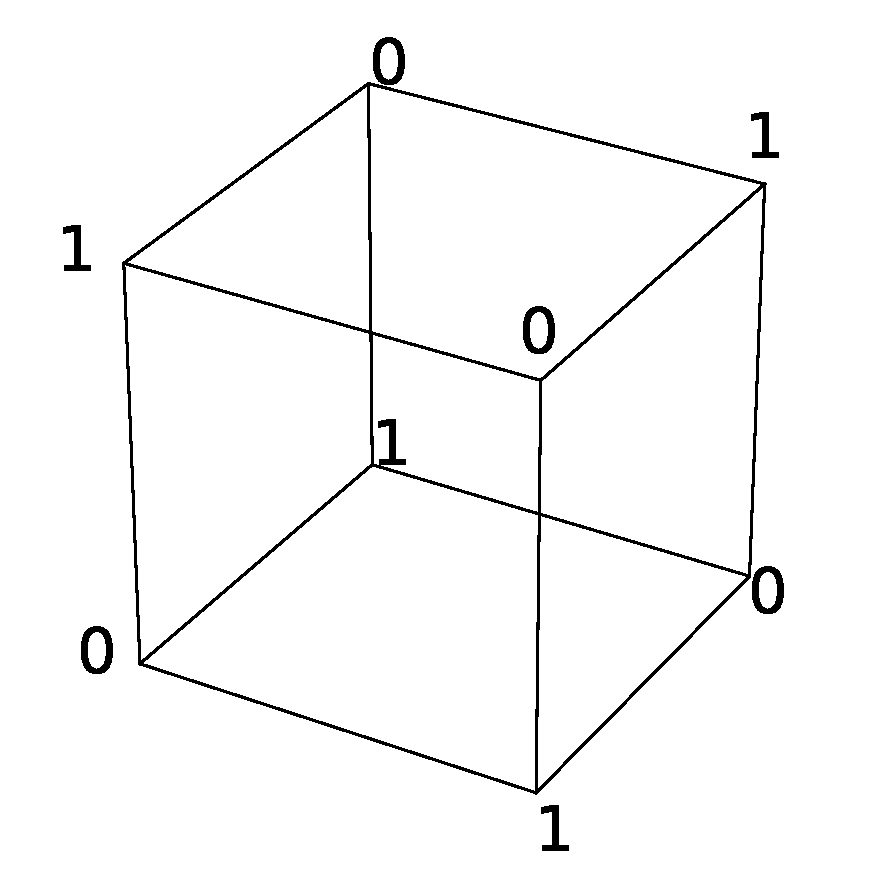
\includegraphics[width=2in]{figures/affine_functions_neighbors.pdf}
  \caption{The labels as determined by the affine function $g(x_1, x_2, x_3) =
  x_1 + x_2 + x_3$. Each $1$ is surrounded by three $0$, and each $0$
  is surrounded by three $1$. Note that solving any (solvable) analogical
  equation leads to the correct solution: this is because $g$ is AP. Also, we
  see that we have here a classification problem that is highly non-linearly
  separable.}
  \label{FIG:affine_functions_neighbors}
\end{figure}

Proposition \ref{PROPOS:affine_functions_are_ap} can now retrospectively
explain the results of Figure \ref{FIG:nan_vs_nn} on page \pageref{FIG:nan_vs_nn}
for the two functions $f_1$ and $f_2$, which are both instances of affine
functions. We saw that for these two functions, $\omegasf$ (defined as the
proportion of elements $\mathbf{x}$ in $\esfs$ for which $\albl{x} = f(x)$) was
always equal to $1$. This result is now obvious and directly comes from the
fact that both $f_1$ and $f_2$ are actually analogy preserving functions: $f_1$
was a projection function while $f_2$ was a general affine function.

We now know that every affine function is AP. We will here give a stronger
result: the affine functions are the \textbf{only} AP functions.  In the
previous subsection, we introduced the ANF of Boolean functions and also
defined their degree. We also mentioned that the class of functions with degree
at most $1$ is exactly the class $L$ of affine functions, which are AP.  We
will show that the class of AP functions is the class of affine functions by
proving that if a function $f$ is AP, then $d(f)\leq 1$. Let us first consider
the case where $d(f) = 2$:

\begin{property} \label{degree_2_not_AP}
 Let $f\colon \mathbb{B}^m\to \mathbb{B}$ with $d(f)=2$. $f$ is not AP.
\end{property}
\begin{proof}
  Let us consider $f$ with $d(f) = 2$ and $\ess(f) \geq 2$. We denote
  $\mathbf{x}_I$ one of the monomial of $f$ of degree $2$. We consider the
  section $f^{\mathbf{0}}_J$, where $J = [1, m] \setminus I$,  and $\mathbf{0}$
  denotes the constant 0 vector in $B^{|J|}$. All variables that are not part
  of the monomial $\mathbf{x}_I$ have been set to $0$. This section
  $f^{\mathbf{0}}_J$ has a unique monomial of degree $2$ (namely
  $\mathbf{x}_I$) and $\ess(f) = 2$.  $f^{\mathbf{0}}_J$ is necessarily
  equivalent to one of the following functions:
  $$
  \begin{cases}
    f_1(x_1, x_2) = x_1 \cdot x_2 + \alpha_0 \\
    f_2(x_1, x_2) = x_1 \cdot x_2 + x_1 + \alpha_0\\
    f_3(x_1, x_2) = x_1 \cdot x_2 + x_1 + x_2 + \alpha_0.
  \end{cases}$$
  To see that none of these functions are AP, consider Table
  \ref{TAB:counter_examples} which gives the values of $f_1, f_2$ and $f_3$
  (with $\alpha_0 = 0$) for the 4-tuple $(\mathbf{a}, \mathbf{b},
  \mathbf{c}, \mathbf{d})$.
  \begin{table}[ht]
    \center
  $\begin{array}{cccccc}
    \toprule
    ~ & x_1 & x_2 & f_1 & f_2 & f_3\\
    \midrule
    \mathbf{a} & 0 & 0 & 0 & 0 & 0\\
    \mathbf{b} & 0 & 1 & 0 & 0 & 1\\
    \mathbf{c} & 1 & 0 & 0 & 1 & 1\\
    \mathbf{d} & 1 & 1 & 1 & 0 & 1\\
    \bottomrule
  \end{array}
  $\bigskip
  \caption{Examples for $f_1, f_2, f_3$ showing that they are not AP.}
  \label{TAB:counter_examples}
  \end{table}
  It is clear that the counter-example $(\mathbf{a},\mathbf{b}, \mathbf{c},
  \mathbf{d})$  shows that $f_1$  is not AP because we have $\mathbf{a} :
  \mathbf{b} :: \mathbf{c} : \mathbf{d}$ and the equation $f_1(\mathbf{a}) :
  f_1(\mathbf{b}) :: f(\mathbf{c}) : y$ is solvable, but the solution is $0$
  while $f(\mathbf{d})$ is $1$. Similarly, $(\mathbf{a},\mathbf{b}, \mathbf{c},
  \mathbf{d})$ is also a counter-example for $f_2$ and $(\mathbf{d},\mathbf{c},
  \mathbf{b}, \mathbf{a})$ is a counter-example for $f_3$.

  As $f_1, f_2, f_3$ are not AP, $f^{\mathbf{0}}_J$ cannot be AP either because
  it is equivalent to one of the $f_i$. As $f^{\mathbf{0}}_J$ is a section of
  $f$, $f$ cannot be AP.
\end{proof}

All we need now is a property that could allow us to decrease the degree of a
function without changing the fact that it is AP. This is the purpose of
Property \ref{section_degree_k_minus_1}.

\begin{property}\label{section_degree_k_minus_1}
Let $f:\mathbb{B}^m\rightarrow \mathbb{B}$ be a function with
  $d(f)=k\geq 2$. Then there is a section $g$ of $f$ with $d(g)=k-1$.
\end{property}
\begin{proof}
Suppose that  $d(f)=k\geq 2$, and let $\mathbf{x}_I$ be a monomial of $f$ of
  maximum degree, i.e. $|I|=k$.  Here again, consider the section $g =
  f^{\mathbf{0}}_J$ where $J = [1, m] \setminus I$ and $\mathbf{0}$ denotes the
  constant $0$ vector in $\mathbb{B}^{|J|}$. It is clear that $g$ is
  represented by a  polynomial that has a unique monomial of maximal degree
  $k$, namely $\mathbf{x}_I$, and maybe some other monomials of degree strictly
  less than $k$.  Let us choose any $i \in I$: then $g' = g^1_{\{i\}}$ is a
  section of $g$ of degree (and arity) $k-1$. As $g'$ is a section of $g$, it
  is also a section of $f$ which completes the proof.
\end{proof}

We are now in position to prove our main result.

\begin{proposition}
  \label{PROPOS:AP_is_L}
The class of AP functions is the class $L$ of affine functions.
\end{proposition}
\begin{proof}
We have seen that every affine function is AP, i.e. if $d(f)\leq 1$, then $f\in
  AP$. On the other hand, Property \ref{degree_2_not_AP} tells us that if
  $d(f)=2$, then $f \notin AP$. So suppose that  $d(f)\geq 3$. By successive
  applications of Property \ref{section_degree_k_minus_1}, it follows that
  there is a section $g$ of $f$ with $d(g)=2$.

  As $g$ is not AP, then $f$ is not AP either. All in all, if $d(f) \geq 2$
  then $f$ is not AP, so the class of AP functions is $L$.
\end{proof}

In the end, we have proved that {\bf the class of functions that ensure a sound
analogical extension of any training set $S \subseteq \mathbb{B}^m$ is the class
of affine functions $L$}. If the function is not affine, then there exists a
training set $S \subseteq \mathbb{B}^m$ for which $\mathbf{E}_S(f)$ is unsound.
We can now finally give a definite answer to our initial problem: \textbf{a
function $f$ is \textit{compatible} with the analogical inference principle if
and only if $f$ is affine.}

In the next subsection, we will focus on some AP functions that are still
\textit{compatible} with the analogical inference principle, but in a stronger
sense.

\subsection{The class of Strongly Analogy Preserving functions.}
\label{SEC:the_class_of_SAP_functions}

Let us come back to the analogical inference principle for a moment, which
states that if we have  $\mathbf{a}: \mathbf{b}:: \mathbf{c}: \mathbf{d}$, then
we should also have $f(\mathbf{a}) :f(\mathbf{b}) :: f(\mathbf{c}) :
f(\mathbf{d})$:
$$
\inferrule{\mathbf{a} : \mathbf{b} :: \mathbf{c} : \mathbf{d}}{ f(\mathbf{a}) :
f(\mathbf{b}) :: f(\mathbf{c}) : f(\mathbf{d}) }
$$
Something we have overlooked so far but that is of importance, is that
implicitly this inference principle requires that the class equation
$f(\mathbf{a}) : f(\mathbf{b}) :: f(\mathbf{c}) : y$ is solvable as soon as we
have $\mathbf{a} : \mathbf{b} :: \mathbf{c} : \mathbf{d}$. Indeed if the
equation is not solvable, then we simply cannot have $f(\mathbf{a}) :
f(\mathbf{b}) :: f(\mathbf{c}) : f(\mathbf{d})$.
Therefore, a more explicit writing of the analogical inference principle is as
follows:
$$
\inferrule[\text{~~ Inference Principle A}]{\mathbf{a} : \mathbf{b} :: \mathbf{c} :
\mathbf{d}}{\solvable(f(\mathbf{a}), f(\mathbf{b}),
f(\mathbf{c})) \\\\f(\mathbf{a}) : f(\mathbf{b}) :: f(\mathbf{c}) :
f(\mathbf{d}) }
$$


Yet, in the end, the ultimate use of this principle is to infer the value of
$f(\mathbf{d})$, and we can only do that by the actual solving of the equation
$f(\mathbf{a}) : f(\mathbf{b}) :: f(\mathbf{c}) : y$ (remember that when we
build the analogical extension, we always require the class equation to be
solvable). This was also the case when we were dealing with the algorithmic
description of the conservative classifier (see e.g. Algorithm
\ref{ALGO:conservative_classifier}).  So if the equation is not
solvable, we are unable to infer anything about $f(\mathbf{d})$. This is why
the AP functions are defined as the functions such that we have $f(\mathbf{a})
:f(\mathbf{b}) :: f(\mathbf{c}) : f(\mathbf{d})$ provided that
$\mathbf{a}: \mathbf{b}:: \mathbf{c}: \mathbf{d}$ stands \textbf{and that}
$f(\mathbf{a}) :f(\mathbf{b}) :: f(\mathbf{c}) : y$ is solvable. With regard to
this, we can say that the class of AP functions is the class of functions that
allow the following inference principle to be sound: $$
\inferrule[\text{~~ Inference principle B}]{\mathbf{a} : \mathbf{b} ::
\mathbf{c} : \mathbf{d} \\\\ \solvable(f(\mathbf{a}), f(\mathbf{b}),
f(\mathbf{c}))}{f(\mathbf{a}) : f(\mathbf{b}) :: f(\mathbf{c}) : f(\mathbf{d})}
$$

\textbf{This one is the inference principle that is actually useful in
practice}: if the
equation is not solvable then we simply try another $4$-tuple. The first one is
too restrictive on the function $f$ because it requires that $\mathbf{a} :
\mathbf{b} :: \mathbf{c} : \mathbf{d} \implies  \solvable(f(\mathbf{a}),
f(\mathbf{b}), f(\mathbf{c}))$, and in practice this requirement is not
needed.

We have shown that the AP functions are those that lead the inference
principle B to be sound.  For the sake of completeness however, we will also
identify the functions that lead the inference principle A to be sound. These
functions will be called Strongly Analogy Preserving functions (SAP):

\begin{definition}[Strongly analogy preserving functions]
  A function $f$ is \textbf{Strongly Analogy Preserving} (SAP) if:
  $$\forall \mathbf{a}, \mathbf{b}, \mathbf{c}, \mathbf{d} \in \mathbb{B}^m, ~~
  \mathbf{a}: \mathbf{b}:: \mathbf{c}: \mathbf{d} \implies
  \begin{cases}
    \text{solvable}(f(\mathbf{a}), f(\mathbf{b}), f(\mathbf{c}))\\
     f(\mathbf{a}) : f(\mathbf{b}) :: f(\mathbf{c}) : f(\mathbf{d}).
  \end{cases}$$
\end{definition}

We will show that the SAP functions are the dictator functions, i.e. functions
of the form $f(\mathbf{x)} = x_i + \alpha_0$ for some $i \in [1, m]$.
Naturally, these are a subclass of affine functions, because every SAP function
is necessarily AP. In Property \ref{PROPER:projections_are_sap}, we prove that
every dictator function  is SAP.

\begin{property}
  \label{PROPER:projections_are_sap}
  Let $f$ be a dictator function, i.e. an affine function of the form:
  $$f(x_1, x_2, \cdots, x_m) = x_i + \alpha_0,$$
  where $i \in [1, m]$ and $\alpha_0 \in \mathbb{B}$. Then $f$ is SAP.
\end{property}
\begin{proof}
  Let $f$ be a dictator function: $f(\mathbf{x}) = x_i$ (we consider $\alpha_0$
  to be $0$ for now). Consider $\mathbf{a}, \mathbf{b}, \mathbf{c}, \mathbf{d}
  \in \mathbb{B}^m$ such that $\mathbf{a}: \mathbf{b}:: \mathbf{c}:
  \mathbf{d}$.

  As the analogy is defined component-wise, this means that we have in
  particular $a_i : b_i :: c_i : d_i$, which is strictly equivalent to
  $f(\mathbf{a}) : f(\mathbf{b}) :: f(\mathbf{c}) : f(\mathbf{d})$, so $f$ is
  SAP. The case where $\alpha_0 = 1$ is derived in the same obvious way.
\end{proof}

It is also easy to show that the two constant functions are SAP. We now show
that the dictators and the constant functions are the only SAP functions:

\begin{proposition}
  The class of SAP functions is the class of dictators and constant functions.
\end{proposition}
\begin{proof}
  We already know that a SAP function is an AP function, so a SAP function
  necessarily is affine. Consider a function $f$ that is affine but that is
  neither a dictator function nor a constant, i.e. $f$ is of the form:
  $$f(\mathbf{x}) = \alpha_1 \cdot x_1 + \cdots +\alpha_m \cdot x_m + \alpha_0,$$
  with at least $\alpha_i = 1$ and $\alpha_j = 1$ for two non-zero indices $i$ and $j$
  with $i\neq j$. Without loss of generality, we will assume that
  $\alpha_0 = 0$.
  Consider now the 4-tuple $(\mathbf{a}, \mathbf{b}, \mathbf{c},
  \mathbf{d})$ such that:
  \begin{itemize}
    \item $a_k = 0$ for all $k \neq i$ and $k\neq j$ ($a_i = a_j = 1$)
    \item $b_k = 0$ for all $k \neq i$ ($b_i = 1$)
    \item $c_k = 0$ for all $k \neq j$ ($c_j = 1$)
    \item $d_k = 0$ for all $k$.
  \end{itemize}

  The 4-tuple is summarized in Table \ref{TAB:SAP}, where we clearly see
  that we have $\mathbf{a} : \mathbf{b} :: \mathbf{c} : \mathbf{d}$, but the
  equation $f(\mathbf{a}) : f(\mathbf{b}) :: f(\mathbf{c}) : y$ is not
  solvable,
  so $f$ is not SAP, QED.

\begin{table}[ht]
  \center
$\begin{array}{cccc}
  \toprule
  ~ & x_i & x_j & f(\cdot) \\
  \midrule
  \mathbf{a} & 1 & 1 & 0\\
  \mathbf{b} & 1 & 0 & 1\\
  \mathbf{c} & 0 & 1 & 1\\
  \mathbf{d} & 0 & 0 & 0\\
  \bottomrule
\end{array}
$\bigskip
\caption{$f$ is not SAP because $f(\mathbf{a}) : f(\mathbf{b}) :: f(\mathbf{c})
  : y$ is not solvable.}
\label{TAB:SAP}
\end{table}

\end{proof}

This section was quite dense, so let us recap a bit what we have seen so far.
We have given two different instances of the analogical inference principle:
$$
\inferrule[\text{~~ Inference Principle A}]{\mathbf{a} : \mathbf{b} ::
\mathbf{c} : \mathbf{d}}{\solvable(f(\mathbf{a}), f(\mathbf{b}),
f(\mathbf{c}))\\\\ f(\mathbf{a}) : f(\mathbf{b}) :: f(\mathbf{c}) :
f(\mathbf{d}) } $$
and
$$
\inferrule[\text{~~ Inference principle B}]{\mathbf{a} : \mathbf{b} ::
\mathbf{c} : \mathbf{d} \\\\ \solvable(f(\mathbf{a}), f(\mathbf{b}),
f(\mathbf{c}))}{f(\mathbf{a}) : f(\mathbf{b}) :: f(\mathbf{c}) : f(\mathbf{d})}
$$

It is obvious that the second version (B) is less restrictive on the function
$f$, and it is the one that is useful in practice. In Section
\ref{SEC:the_class_of_AP_functions}, we showed that the inference principle B
is sound if and only if $f$ is an affine Boolean function. We also showed in
Section \ref{SEC:the_class_of_SAP_functions} that the inference principle A
is sound for dictator functions (a particular case of affine functions).

These are strong theoretical results, but obviously real-world problems are not
limited to the Boolean case, and the function $f$ underlying the labels of a
classification problem is almost never completely affine. We will address these
issues in the next section.

\section{Beyond Boolean Analogy Preserving functions}
\label{SEC:beyond_boolean_AP_functions}

The aim of this section will be to complement the theoretical results of
Section \ref{SEC:a_complete_characterization_of_AP_functions}. We will first
stay in the Boolean setting in Section \ref{SEC:approximate_ap_functions}
and empirically study the behaviour of functions that  are \textit{close} from
being AP. In Sections \ref{SEC:extension_to_nominal_attributes} and
\ref{SEC:extension_to_real_valued_functions}, we will derive some more
theoretical results about AP functions when dealing with nominal values and
with real values.

\subsection{Approximately AP functions and experiments}
\label{SEC:approximate_ap_functions}

While the theoretical result of Proposition \ref{PROPOS:AP_is_L} is interesting
on its own, it is obvious that purely affine functions are not representative
of what would be encountered in a real-world Boolean environment.  This leads to the
following question: what remains of the quality of the analogical extension
$\mathbf{E}_S(f)$ when $f$ deviates from being AP in different ways? We will
here investigate this question.

\paragraph{$\varepsilon$-close functions from $L'$\\}

Recall that for a given training $S$, we defined $\omegasf$ as the quality of the
extension $\esf$ with $\omegasf \eqdef P\left(\albl{\mathbf{x}} = f(\mathbf{x})
\given[\big] \mathbf{x} \in \esfs\right).$ By definition, $\omegasf=1$ for all
$S$ iff $f$ is AP. What we want to know now is how $\omegasf$ is affected when
$f$ is not a purely affine function. What we
mean by \textit{not purely affine} is that $f$ is at a distance at most
$\varepsilon$ from the set
of affine functions. We will define these notions now.

Given two Boolean functions $f$ and $g$, we define their distance
$\text{dist}(f, g) \eqdef P\left(f(\mathbf{x}) \neq
g(\mathbf{x})\right)$, where $P$ is the uniform distribution over
$\mathbb{B}^m$. Here, $\mathbf{x} \in \mathbb{B}^m$ is also considered as a
random variable.

\begin{definition}[$\varepsilon$-close functions]
We say that $f$ is $\varepsilon$-close to $g$ if $\text{dist}(f, g) \leq
  \varepsilon$, and that $f$ is $\varepsilon$-close to a set of functions $\Sigma$ if
  $\exists g \in \Sigma$ such that $f$ is $\varepsilon$-close to $g$.
\end{definition}

We want to study here the value of $\omegasf$ when $f$ is $\varepsilon$-close from
$L$, the set of affine functions. Note however that thanks to the
code-independency property of the Boolean proportion ($1$ and $0$ play
symmetric roles), we have that for any $S$ and any $f$, $\omegasf =
\omega_S^{\neg f}$. As the set of affine functions is the set of linear
functions and their negations, \textbf{it is enough to study the value of
$\omegasf$ when $f$ is $\varepsilon$-close to $L'$, the set of linear functions}.

This question is clearly of interest, because in practice there exists some
statistical test allowing the practitioner to query a partially-known function
$f$ to find out if it is $\varepsilon$-close to $L'$. This test is the BLR test
\cite{BluLubRub93}, whose steps are as follows:

\begin{itemize}
\item Choose randomly and independently $\mathbf{x}$ and $\mathbf{y}$ in
  $\mathbb{B}^m$.
\item Compute $f(\mathbf{x}+\mathbf{y})$ and $f(\mathbf{x}) + f(\mathbf{y})$.
\item If $f(\mathbf{x}+\mathbf{y}) = f(\mathbf{x}) + f(\mathbf{y})$, return
  \textit{Accept}.
\end{itemize}

The main useful result is given in Property \ref{PROPER:BLR_test}:
\begin{property}
  \label{PROPER:BLR_test}
  If $BLR$ accepts $f$ with a probability at least $1-\varepsilon$, then $f$ is
  $\varepsilon$-close to the set of linear functions $L'$.
\end{property}

So if we can exhibit a clear probabilistic dependence between $\omegasf$
and $\varepsilon$, this would allow the practitioner to have guarantees about
$\omegasf$ because we can know $\varepsilon$ from the BLR test.

Let us first consider the following experiment. Starting from a linear function $g
\colon \mathbb{B}^8 \to \mathbb{B}$ defined as  $g(\mathbf{x}) = x_1 + \cdots +
x_8$, we introduce some noise by negating its output $g(\mathbf{x})$ with
probability $\varepsilon$. We thus obtain some functions $f_{\varepsilon}$ that are
$\varepsilon$-close to $L'$, and report the value of $\omega_S^{f_\varepsilon}$ averaged over $50$
experiments.  Figure \ref{omega_vs_eps} gives an
illustration of the variation of $\omega_S^{f_\varepsilon}$ (simply denoted
$\omega$) against  $\varepsilon$ for different
sizes of $S$ (as a percentage of $|\mathbb{B}^m|$).  Other experiments have
been carried out with other affine functions (i.e.  with less essential
variables or different arity), leading to very similar results. As a side note,
$\varepsilon$ only needs to be taken in $[0, \frac{1}{2}]$, because $f_\varepsilon =
\neg f_{1 - \varepsilon}$ and for any $f$, we have $\omegasf = \omega_S^{\neg
f}$.

\begin{figure}
\begin{center}
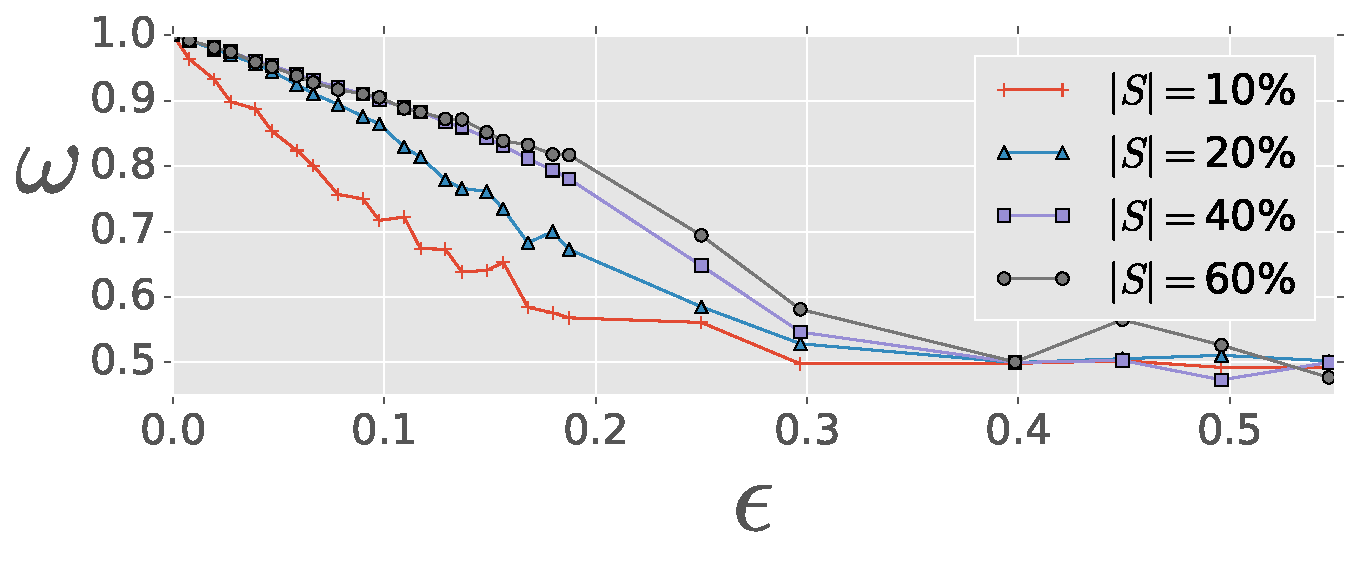
\includegraphics[scale=0.6]{figures/omega_vs_eps_dim8_nexp50_std_nEss8.pdf}
  \caption{$\omega$ for $\varepsilon$-close functions to $L$.}
\label{omega_vs_eps}
\end{center}
\end{figure}

When $\varepsilon = 0$, i.e. when $f_\varepsilon$ is AP, we get $\omega = 1$ as expected from
Proposition \ref{PROPOS:AP_is_L}. We observe an almost linear decrease in $\omega$ as
$\varepsilon$ grows to $0.3$ then leading to a plateau where $\omega =
\frac{1}{2}$, indicating that the analogical labels $\albl{\mathbf{x}}$ are
more or less random. Moreover, $\omega$ appears to decrease faster for small
training set $S$. This is due to the fact that the analogical labels
$\albl{\mathbf{x}}$ are the result of a majority-vote procedure among the
candidate solutions that one can build from $S$, and the number of candidates
becomes smaller as $\mid S\mid$ decreases, thus altering the quality of the
prediction.

We only have an empirical study here. Ultimately, it would be very interesting
to prove a result like
$$P(\omegasf \geq \eta) > 1 - \delta,$$
where $\eta \in [0, 1]$ and $\delta \in [0, \frac{1}{2}]$ are parameters 
depending on $\varepsilon$ and $\mid S \mid$. Such a result would be strongly
linked to the PAC learning theory \cite{Val72}, and is the object of current
research.

\paragraph{Other non-AP functions\\}


We have studied so far the variation of $\omegasf$ when $f$ deviates from
the set of affine functions. We now focus on another point: the variation of
$\omegasf$ when $f$ deviates from being AP in a different way.
Let us note the following point: even though a function $f$ is far from being
AP, the quality $\omegasf$ of the extension $\esf$ may still be very
high. To illustrate this, let us define the value $\beta$ which is an indicator
of how far is $f$ from being completely AP.  For each $\mathbf{x} \in
\esfs$, we define $\beta_\mathbf{x}$ as the proportion of
candidates $\sol(f(\mathbf{a}), f(\mathbf{b}), f(\mathbf{c}))$ (with
$(\mathbf{a}, \mathbf{b}, \mathbf{c}) \in \rsfx$) that led to the correct
label, i.e. the proportion of candidate solutions that are equal to
$f(\mathbf{x})$. $\beta$ is defined as the average of all the
$\beta_\mathbf{x}$.  Obviously, a function $f$ is AP iff $\beta = 1$ for all
$S$, i.e. iff $\beta_\mathbf{x} = 1$ for all $\mathbf{x} \in \esfs$
and for all $S$.

Table \ref{table_monks} reports the values of $\omega$ and $\beta$ over three
datasets from the UCI repository, namely the three Monk's problems\footnote{As
these datasets are nominally-valued, they have been binarized.} \cite{UCIrepo}.
Results are averaged over 100 experiments, where the training set $S$ is each
time randomly sampled with a size of $30$\% of the universe of possible
instances.

\begin{table}
\centering
\begin{tabular}{ c  c  c }
\toprule
  & $\omega$  & $\beta_S$ \\
\midrule
Monk 1 & .96 & .73 \\
Monk 2 & .96 & .69 \\
Monk 3 & .98 & .87 \\
\bottomrule
\end{tabular}
\caption{$\omega$ and $\beta$ over the Monk's problems.}
\label{table_monks}
\end{table}

We observe that for each dataset, $\beta$ is significantly lower than $1$.
This suggests that the Boolean functions underlying these datasets are highly
not AP, because on average, there is a high proportion (around $20$\%) of
candidates that predicted the wrong label. However, $\omega$ is not lower than
$96$\%, implying extensions of very high quality.  \textbf{This is where the
majority-vote comes into play}: in some cases, it may be able to compensate for
the predictors that were wrong.  This is what happens here in $96$\%, $96$\%
and $98$\% of the cases respectively. Here again, obtaining theoretical
guarantees about the majority-vote procedure is currently investigated.

In the next subsection, we will extend our theoretical results about Boolean AP
functions to a more general setting where instances are nominally valued.

\subsection{Extension to nominal attributes}
\label{SEC:extension_to_nominal_attributes}

When it comes to real life applications, it is quite rare to get a purely
Boolean dataset.  It is generally the case that the dataset  is  a mix between
Boolean attributes and nominal attributes taking their values in finite sets.
For instance, an attribute \textit{color} typically takes its values in, let us
say, $\Set{red, green,blue}$. Unfortunately, on this set of values for attribute
\textit{color}, there is no structure, no order and no known operator.
Nevertheless, there is still a way to deal with such attributes within the
analogical framework, and to characterize AP functions in such settings. This
is what we will investigate in this subsection.
 

We have already seen in Chapter \ref{CHAP:formal_analogical_proportions} that we
can define an analogical proportion on a set $X$ by restricting the accepted
analogical patterns to $a:b::a:b$ and $a:a::b:b$.  Formally, an analogy $A$
over $X$ is a subset of $X^4$ defined as:
$$A \eqdef \Set{ (a,a,b,b)  | a, b \in X} \cup \Set{ (a,b,a,b) | a, b \in X}.$$

Back to the \textit{color} attribute, it means that we consider
$red:blue::red:blue$ as a valid analogical proportion but $red:blue::red:green$
is not valid. We can easily extend component-wise this analogy to a Cartesian
product $X^m=\prod_{i=1}^m X_i$ which is now equipped with an analogical
relation. In classification, this allows to deal with any kind of nominal
attributes.  In this setting, a binary classification function $f$ is a
function from $X^m=\prod_{i=1}^m X_i$ to $\mathbb{B}$. The question we want to
address here is the same as that of Section
\ref{SEC:a_complete_characterization_of_AP_functions}: we want to characterize all
the functions $f$ that lead to a perfectly sound analogical extension.
Unfortunately, we cannot turn to the previous framework because the Cartesian
product $X^m$ is made of distinct sets and is not a power of
$\mathbb{B}$ anymore. So we will not be able to entirely identify these functions,
simply because we do not even know how to \textit{write} them. When dealing
with Boolean functions we used an algebraic point of view that allowed us
to write the functions in their Algebraic Normal Form, and we identified the AP
functions as those that have a particular ANF. But this will not be
possible here, because there is no algebraic structure on the Cartesian product that
is the domain of our functions.

Nonetheless, we will still find close links between the AP Boolean functions
and the AP functions of our current setting, and these links are based on the
\textit{binarization} of the nominal attributes. Indeed, any nominal attribute
with $k$ values can be binarized into $k$ Boolean attributes. We can also choose
$k- 1$ attributes, or some other fancy binarization procedure, but we will
stick to the simplest one:
binarizing the \textit{color} attribute leads to three binary attributes
$(is\_red, is\_green, is\_blue)$ so that $red$ is coded as $(1, 0, 0)$,
$green$ is coded as $(0, 1 , 0)$ and $blue$ is coded as $(0, 0, 1)$. Obviously,
the $k$ Boolean attributes are not independent: for example $(1, 1, 1)$  is not
a valid value.  More formally, let us denote $\bin$ this injective embedding
going from $X_i=\{v_1, \dots, v_k\}$ to $\mathbb{B}^k$:
$$\bin(v_i) \eqdef (0, \dots, 0, 1, 0, \dots 0),$$
where $1$ is at position $i$.  So if we have a set of nominal attributes $x_1,
\dots, x_m$ where $x_i$ takes its values in a finite set $X_i$, the Cartesian
product  $\prod_{i=1}^m X_i$ can be mapped into the set $\prod_{i=1}^m
\mathbb{B}^{\mid X_i \mid}$ by applying the injective embedding $\bin$ in a
component-wise fashion:
$$\bin(\prod_{i=1}^m X_i) \eqdef \prod_{i=1}^m  \bin(X_i).$$

From the very definition of this embedding, we have the following immediate and
obvious property:
\begin{property}
  \label{PROPER:analogy_nominal_iff_analogy_bin}
  For any $\mathbf{a}, \mathbf{b}, \mathbf{c}, \mathbf{d} \in X^m =
  \prod_{i=1}^m X_i$,
$$\mathbf{a}: \mathbf{b}:: \mathbf{c}: \mathbf{d} \iff
 \bin(\mathbf{a}): \bin(\mathbf{b}):: \bin(\mathbf{c}):
  \bin(\mathbf{d}).$$
 \end{property}
 \noindent
 Note that the proportion $\mathbf{a}: \mathbf{b}:: \mathbf{c}: \mathbf{d}$
 holds in $X^m$ while the proportion $\bin(\mathbf{a}): \bin(\mathbf{b})::
 \bin(\mathbf{c}): \bin(\mathbf{d})$ is a usual Boolean proportion that holds
 in $\prod_{i=1}^m\mathbb{B}^{\mid X_i \mid}$.  Now, every function $f$ from
 $\prod_{i=1}^n X_i$ to $\mathbb{B}$ can be associated to a \textbf{partial}
 Boolean function $f^b$ from $\prod_{i=1}^m \mathbb{B}^{|X_i|}$ to $\mathbb{B}$
 where $f^b$ is defined as follows:
$$
f^b(\bin(\mathbf{x})) \eqdef f(\mathbf{x}).
$$

As the initial nominal universe  $\prod_{i=1}^m X_i$  has been compiled into a
Boolean universe, it is tempting to consider the framework that has been
developed in Section \ref{SEC:a_complete_characterization_of_AP_functions}.
Unfortunately, the whole set $\prod_{i=1}^m \mathbb{B}^{\mid X_i\mid}$ is not
the exact image of $\prod_{i=1}^m X_i$: it is bigger, and some elements in
$\prod_{i=1}^m  \mathbb{B}^{\mid X_i\mid}$ are not the image of an element of
$\prod_{i=1}^m X_i$ using $\bin$.  Ultimately, the domain of $f^b$ is just
$\bin(\prod_{i=1}^m X_i)$, which is included in $\prod_{i=1}^m
\mathbb{B}^{|X_i|}$. This is why $f^b$ is considered to be a partial function.

Nevertheless, the AP property is still relevant for functions that are only
partially defined: a partially defined function that always leads to a perfectly
sound analogical extension for any training set $S$ will also be said to be
Analogy Preserving, and will be called PAP for Partial AP. Just like in Section
\ref{SEC:a_complete_characterization_of_AP_functions}, a natural way to
characterize PAP functions is given in Definition \ref{DEF:PAP_functions}:

\begin{definition}[Partial analogy preserving functions]
  \label{DEF:PAP_functions}
  A \textbf{partial} function $f^b$ is {\bf Analogy Preserving} (PAP)
  if for all $\mathbf{a}, \mathbf{b}, \mathbf{c}, \mathbf{d} \in
  \text{dom}(f^b)$:
  $$
  \begin{cases}
    \mathbf{a} :  \mathbf{b} ::  \mathbf{c} :  \mathbf{d} \text{ and }\\
    solvable(f^b(\mathbf{a}),f^b(\mathbf{b}),f^b(\mathbf{c}))
  \end{cases}
  \implies \text{sol}(f^b(\mathbf{a}),f^b(\mathbf{b}),f^b(\mathbf{c})) =
  f^b(\mathbf{d}).
  $$
\end{definition}

Proposition \ref{PROPOS:PAP_eq_AP} will provide us with the link between $f$
and $f^b$, when one of them is AP:

\begin{proposition}
  \label{PROPOS:PAP_eq_AP}
Let $f$ be a function from $\prod_{i=1}^n X_i$ to $\mathbb{B}$. Then $f$ is AP
if and only if $f^b$ is PAP.
\end{proposition}
\begin{proof}
  Let us assume that $f$ is AP and let be 4 elements belonging to the domain of
  $f^b$: $\bin(\mathbf{a}),\bin(\mathbf{b}), \bin(\mathbf{c}), \bin(\mathbf{d})
  \in \bin(\prod_{i=1}^m X_i)$ such that:
  $$\begin{cases}
    \bin(\mathbf{a}):\bin(\mathbf{b})::\bin(\mathbf{c}):\bin(\mathbf{d}) \mbox{
      and}\\
    \solvable(f^b(\bin(\mathbf{a})),f^b(\bin(\mathbf{b})),f^b(\bin(\mathbf{c}))).
  \end{cases}
  $$
Thanks to Property \ref{PROPER:analogy_nominal_iff_analogy_bin}, we have seen
  that in this case we also have
  $\mathbf{a}:\mathbf{b}::\mathbf{c}:\mathbf{d}$.  Since by definition
  $f(\mathbf{x}) = f^b(\bin(\mathbf{x}))$,  the second condition simply is
  $\solvable(f(\mathbf{a}),f(\mathbf{b}),f(\mathbf{c}))$. As $f$ is AP,
  $\sol(f(\mathbf{a}),f(\mathbf{b}),f(\mathbf{c}))= f(\mathbf{d})$, and
  $f(\mathbf{d}) = f^b(\bin(\mathbf{d}))$. So in the end, we have that
  $\sol((f^b(\mathbf{a}),f^b(\mathbf{b}),f^b(\mathbf{c})) =
  f^b(\bin(\mathbf{d}))$, which proves that $f^b$ is PAP.

  Let us now focus on the reverse implication. Consider a PAP function
  $f^b$ and 4 elements $\mathbf{a}, \mathbf{b}, \mathbf{c}, \mathbf{d} \in
  \prod_{i=1}^m X_i$ such that:
  $$
  \begin{cases}
  \mathbf{a}:\mathbf{b}::\mathbf{c}:\mathbf{d} \mbox{ and}\\
  \solvable(f(\mathbf{a}),f(\mathbf{b}),f(\mathbf{c})).
  \end{cases}
  $$
  Thanks again to Property \ref{PROPER:analogy_nominal_iff_analogy_bin},
  $\bin(\mathbf{a}):\bin(\mathbf{b})::\bin(\mathbf{c}):\bin(\mathbf{d})$ holds. 
  The second condition is just
  $\solvable(f^b(\bin(\mathbf{a})),f^b(\bin(\mathbf{b})),f^b(\bin(\mathbf{c})))$
  because by definition $f(\mathbf{x}) = f^b(\bin(\mathbf{x}))$. Because
  $f^b$ is PAP, we have that
  $\sol(f^b(\bin(\mathbf{a})),f^b(\bin(\mathbf{b})),f^b(\bin(\mathbf{c}))) =
  f^b(\bin(\mathbf{d}))$. As $f^b(\bin(\mathbf{d}))=f(\mathbf{d})$ by
  definition, we have that $f$ is AP.
\end{proof}

In the end, the notion of AP function is smoothly transferable to the notion
of PAP function. This result is only purely theoretical, and sadly there is  
not much more we can extract from it for practical use. Proposition
\ref{PROPOS:PAP_eq_AP} tells us that when dealing with nominal attributes, if
the function underlying the ground truth labels is affine once the dataset has
been binarized, then we can safely extend our training set. As
there are no common operators on the set  $\prod_{i=1}^n X_i$, we are not able
to give a more accurate characterization of AP functions in such settings.

In the next subsection, however, we will see that in a real setting the AP
functions are also precisely the affine (real) functions.

\subsection{Extension to real-valued functions}
\label{SEC:extension_to_real_valued_functions}

Section \ref{SEC:a_complete_characterization_of_AP_functions} was devoted to the
identification of Boolean functions that were fully compatible with the
analogical inference principle, and we saw that
these functions are the Boolean affine functions. One may wonder what would
these functions be in a real setting, i.e. using functions  from $\mathbb{R}^m$
to $\mathbb{R}$ with the arithmetic proportion?

Well, we already know that the Boolean proportion and the arithmetic proportion
are really close. Once again, we will witness this close bond: in a real
setting, the class of AP functions is also the class of real affine functions.
Luckily, the proof is a lot easier to derive.  Let us first (re)define the
arithmetic proportion:
\begin{property}
  \label{PROPER:sol_arithm_prop}
  Four elements $\mathbf{a}, \mathbf{b}, \mathbf{c}, \mathbf{d} \in
  \mathbb{R}^m$ are in arithmetic proportion if $\mathbf{d} = \mathbf{c} -
  \mathbf{a} + \mathbf{b}$.

  Also, for any $a, b, c \in \mathbb{R}$, the equation $a : b :: c:y$ is always
  solvable and the solution is $\emph{sol}(a, b, c) = c - a + b$.
\end{property}

Please note that here, $+$ is the regular addition operator (not the
modulo-2 addition as in the previous sections). We will also use a simple property of
affine functions:

\begin{property}
  \label{PROPRE:f_affine_real}
  A real function $f$ from $\mathbb{R}^m$ to $\mathbb{R}$ is affine if f is of
  the form: $$f(\mathbf{x}) = \boldsymbol{\alpha} \cdot \mathbf{x} +
  \alpha_0,$$
  where $\boldsymbol{\alpha} \in \mathbb{R}^m$, $\alpha_0  = f(\mathbf{0})
  \in \mathbb{R}$, and $\cdot$ is here the usual dot product.  Also, $f$ is affine iff $\forall \mathbf{a}, \mathbf{b},
  \mathbf{c} \in
  \mathbb{R}^m$:

  $$f(\mathbf{c} - \mathbf{a} + \mathbf{b}) = f(\mathbf{c}) - f(\mathbf{a}) +
  f(\mathbf{b}).$$
\end{property}
\begin{proof}
  Let $f$ be an affine function.
  $\forall \mathbf{a}, \mathbf{b}, \mathbf{c} \in \mathbb{R}^m$,
  \begin{align*}
    f(\mathbf{c} - \mathbf{a} + \mathbf{b}) &= \boldsymbol{\alpha} \cdot (\mathbf{c}
    - \mathbf{a} + \mathbf{b}) + \alpha_0\\
    &= \boldsymbol{\alpha} \cdot \mathbf{c} - \boldsymbol{\alpha} \cdot
    \mathbf{a} + \boldsymbol{\alpha} \cdot \mathbf{b} + \alpha_0\\
    &= f(\mathbf{c}) - f(\mathbf{a}) + f(\mathbf{b}).
  \end{align*}

  Now, let $f$ be a function such that $f(\mathbf{c} - \mathbf{a} +
  \mathbf{b}) = f(\mathbf{c}) - f(\mathbf{a}) + f(\mathbf{b})$, and consider
  the function $g$ defined by $g(\mathbf{x}) = f(\mathbf{x}) - f(\mathbf{0}).$
  \begin{align*}
    g(\mathbf{x} + \mathbf{y}) &= f(\mathbf{x} + \mathbf{y}) - f(\mathbf{0})\\
    &= f(\mathbf{x} - \mathbf{0} + \mathbf{y}) - f(\mathbf{0})\\
    &= f(\mathbf{x}) + f(\mathbf{y}) - 2f(\mathbf{0})\\
    &= g(\mathbf{x}) + g(\mathbf{y}).
  \end{align*}

  So $g(\mathbf{x} + \mathbf{y}) = g(\mathbf{x)} + g(\mathbf{y})$ and by
  definition, $g$ is linear and can be written as:
  $$g(\mathbf{x}) = \boldsymbol{\alpha} \cdot \mathbf{x}.$$

  So $f(\mathbf{x}) = \boldsymbol{\alpha} \cdot \mathbf{x} + f(\mathbf{0}),$
  which makes $f$ affine.
\end{proof}

We will now prove that the real AP functions are the real affine functions, just
like the Boolean AP functions are the Boolean affine functions.

\begin{proposition}
  \label{PROPOS:arithm_AP_func_affine_func}
  With the arithmetic proportion, the set of real AP functions from
  $\mathbb{R}^m$ to $\mathbb{R}$ is the set of affine functions.
\end{proposition}
\begin{proof}
  A real function $f$ is AP iff for all $\mathbf{a}, \mathbf{b}, \mathbf{c},
  \mathbf{d} \in \mathbb{R}^m$,

  $$\mathbf{a}: \mathbf{b}:: \mathbf{c}: \mathbf{d} \implies
  \sol(f(\mathbf{a}), f(\mathbf{b}), f(\mathbf{c})) = f(\mathbf{d}).$$

  Equivalently, thanks to property \ref{PROPER:sol_arithm_prop},  $f$ is AP
  iff: $$\mathbf{d} = \mathbf{c} - \mathbf{a} + \mathbf{b} \implies
  f(\mathbf{c}) - f(\mathbf{a}) +  f(\mathbf{b}) = f( \mathbf{c} - \mathbf{a} +
  \mathbf{b}).$$

  From Property \ref{PROPRE:f_affine_real}, this is true iff $f$ is affine.
\end{proof}

Proposition \ref{PROPOS:arithm_AP_func_affine_func} is illustrated in Figure
\ref{FIG:real_AP_func}.
\begin{figure}[!h]
\centering
  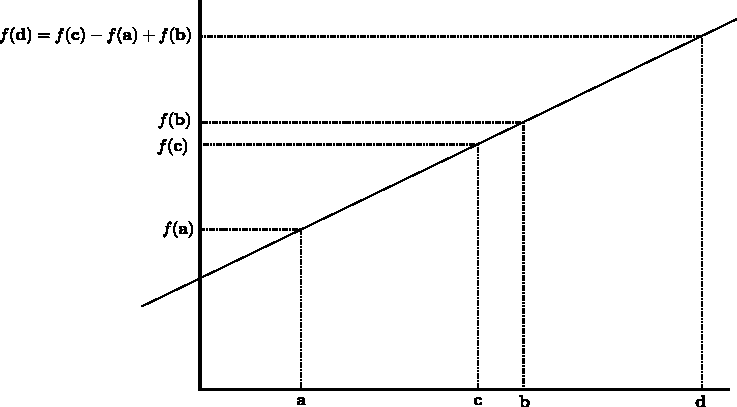
\includegraphics[width=3.5in]{figures/real_AP_fuction.pdf}
  \caption{When $f$ is affine, $\sol(f(\mathbf{a}), f(\mathbf{b}),
  f(\mathbf{c})) = f(\mathbf{d})$.}
\label{FIG:real_AP_func}
\end{figure}

In fact, Proposition \ref{PROPOS:AP_is_L} for Boolean functions can be
proved in a much simpler way than what was used in Section
\ref{SEC:a_complete_characterization_of_AP_functions}, using
the same outline as Proposition \ref{PROPOS:arithm_AP_func_affine_func}. The
first step is to see that a Boolean function is affine iff $f(\mathbf{a} +
\mathbf{b} + \mathbf{c}) = f(\mathbf{a}) + f(\mathbf{b}) + f(\mathbf{c})$,
where $+$ is now the modulo-2 addition. Also, noting that $\mathbf{a} :
\mathbf{b} :: \mathbf{c} : \mathbf{d} \implies \mathbf{d} = \mathbf{a} +
\mathbf{b} + \mathbf{c}$ and that for any $a, b, c \in \mathbb{B}$ we have
$\sol(a, b, c) = a + b + c$, the proof can be derived easily. We chose to give
the longest one in Section
\ref{SEC:a_complete_characterization_of_AP_functions} because this is the one
that was originally derived (plus, it was the one that was used in our
publication \cite{CouHugPraRicIJCAI17}).

\section*{Conclusion}

The main contribution of this chapter was to provide a complete
characterization of Boolean functions that are fully compatible with the
analogical inference principle that we have used so far in all the previous
chapters of this document. Using an appropriate representation for Boolean
functions (namely their algebraic normal form), we have been able to prove that
the class of AP functions is the class of affine functions, i.e. functions
whose degree is less than $1$.

We have chosen to tackle the problem of finding the class of AP functions from the
angle of training set extension. It became clear that the class of AP functions
can be seen as the class of functions which allow  a perfectly sound extension,
or equivalently as the class of functions which allow the analogical inference
principle to be sound.

We also provided a more explicit version of the analogical inference principle
which is in fact less restrictive than the one we had claimed so far. The
distinction between the strict version and the relaxed version is that the
class equation $f(\mathbf{a}) : f(\mathbf{b}) ::f(\mathbf{c}) :y$ is not always
solvable, and the relaxed version takes this fact into account. The class of AP
functions is fully compatible with the relaxed version, but we have also
identified the functions that are compatible with the strict version, which
turned out to be the class of projection (or dictator) functions.

In real-world application though, purely affine functions are extremely rare.
This means that using the analogical inference principle will necessarily
produce errors in the label predictions. We have empirically investigated the
quality of the analogical extension (which measures in some sense how
\textit{adequate} was the use of the analogical inference principle) when a
function deviates from the class of purely affine functions. We have observed
that the quality of the extension linearly decreases, but a strong statistical
result still needs to be derived. We also noted that in some particular cases,
a function that is strongly not AP can still lead to a high extension quality.
Indeed, as the analogical labels are the result of a majority-vote procedure,
it may happen that the most common candidate label actually corresponds to the
ground truth label $f(\mathbf{x})$. In this case, the majority-vote procedure
is able to compensate for the candidates that were wrong in their predictions,
because it will choose the most common predictor that happens to be the
correct label.  Ultimately, even if only $50\% + \varepsilon$ ($\varepsilon > 0$) of
the candidates are correct, it is still enough to have a perfectly sound
extension. The class of AP functions ensures that exactly $100\%$ of the
candidates are correct, but it is clear that such a requirement is too strong
to be really useful in practice. The derivation of a theoretical result
involving the role  of the majority-vote procedure is still a topic of current
research.

Our main goal was to identify the class of AP functions in a Boolean setting.
We have extended our results to two other domains. It is often the case that
the classification problem does not involve purely Boolean attributes, but
rather a more general domain where instances are multi-valued. Sadly in these
domains, there is no known structure or operators, so it was not possible to
give a clear identification of AP functions such as that of Boolean AP
functions. We were however able to provide a clear link between these AP
functions and the Boolean AP functions by embedding the multi-valued space
into a partially defined Boolean space. We also provided a clear identification
of AP functions in a real setting, i.e. for functions from $\mathbb{R}^m$ to
$\mathbb{R}$. It turns out that the class of real AP functions is the class of
real affine functions, just like the class of Boolean AP functions is the class
of Boolean affine functions. The result for real functions was much easier to
prove and in the end quite trivial, and seems to strongly limit the use of the
analogical inference principle in a real setting.
